% A simple LaTeX template for lab reports in TDT4258 Energy Efficient Computer Design
% by Yaman Umuroglu (yamanu@idi.ntnu.no)
% Feel free to customize the style as you see fit, but the chapters/sections mentioned in the
% template should be included with the appropriate content.

\documentclass[abstract=on]{scrreprt}
\usepackage[utf8]{inputenc}


\usepackage{natbib}
\usepackage{graphicx}
\usepackage{textcomp}
\usepackage{amsmath}
\usepackage{listings}
\usepackage{url}
\usepackage{color}
\usepackage{float}
\usepackage[titletoc]{appendix}
\definecolor{lightgray}{rgb}{0.9,0.9,0.9}

\lstset{
    basicstyle=\footnotesize\ttfamily, % Standardschrift
    numbers=left,               % Ort der Zeilennummern
    numberstyle=\tiny,          % Stil der Zeilennummern
    %stepnumber=2,               % Abstand zwischen den Zeilennummern
    numbersep=5pt,              % Abstand der Nummern zum Text
    tabsize=2,                  % Groesse von Tabs
    extendedchars=true,         %
    breaklines=true,            % Zeilen werden Umgebrochen
    keywordstyle=\color{red},
    frame=b,         
 %  keywordstyle=[1]\textbf,    % Stil der Keywords
 %  keywordstyle=[2]\textbf,    %
 %  keywordstyle=[3]\textbf,    %
 %  keywordstyle=[4]\textbf,   \sqrt{\sqrt{}} %
    stringstyle=\color{blue}\ttfamily, % Farbe der String
    showspaces=false,           % Leerzeichen anzeigen ?
    showtabs=false,             % Tabs anzeigen ?
    xleftmargin=17pt,
    framexleftmargin=17pt,
    framexrightmargin=5pt,
    framexbottommargin=4pt,
    backgroundcolor=\color{lightgray},
    showstringspaces=false      % Leerzeichen in Strings anzeigen ?        
}

% Edit the meta.tex file to change title, group number and author names
% Fill in the report title, group number and student names here
\newcommand{\mytitle}{Vector Graphics Processor}
\newcommand{\myauthor}{Anders Lima\\Jonatan Lund\\Øyvind Robertsen\\Håvard Holmboe Lian\\Jonas Halland\\Christian De Frene\\Helmer Njærheim}

\title{\mytitle}
\author{\myauthor}
\date{\today}



\begin{document}
% The title page, edit if you want to customize it
\begin{titlepage}

\includegraphics[height=3cm]{images/ntnu_logo.pdf}\\[1cm]   

\begin{center}
 
% Upper part of the page
~\\[1.5cm]

\textsc{\Large TDT4295 Computer Design Project}\\[0.5cm]

% Set the title of the Document between two horizontal lines
\hrule ~\\[0.2cm]
{\huge \bfseries \mytitle}\\[0.9cm]		% print the title of the document
\hrule ~\\[1.5cm]

% Additional Information about the document
\begin{minipage}{0.4\textwidth}
    \centering
	\large
		\myauthor
\end{minipage}

\vfill

% Bottom of the page
{\large \today}

\end{center}
\end{titlepage}


% Main matter - edit corresponding file under content/ to change
\begin{abstract}

\end{abstract}
\tableofcontents

% Part I
\part{Introduction}
\chapter{TDT4295 - Computer Design Project}
\label{sec:intro}

The Computer Design Project is held at NTNU every fall.
It is a large, project-based subject in which students create a working computing platform, more or less from scratch.
This year saw high enough participation that two assignments were presented, and two groups formed around these.
The report you're now reading details the work done and solution implemented by the vector graphics processor group.

This chapter introduces the project, describes the requirements, outlines the solution and provides a fundamental understanding of vector graphics. It ends with

\section{Assignment}

This year's assignment focuses on graphics, exploring both of the traditional ways of representing and processing graphics: raster-based and vector-based.
Two distinct assignment texts were presented by the course staff: one focusing on raster-based graphics, the other on vector graphics.
The following is a verbatim copy of the vector graphics assignment text \cite{assignment-text}.

\subsection{Assignment Text - A Vector Graphics Processor}

Image generation using vector graphics as the core method is a powerful and scalable way of generating image data.
Vector graphics represents images at a higher abstraction level than single-pixels.
A vector graphics processor can make use of drawing instructions to produce images, which is a task well suited for hardware acceleration \cite{openvg}.
Parallelization with multiple cores and/or at the instruction level are architectural possibilities that can be exploited to design a specialized processor.
The task is to design and implement a processor for producing vector graphics.
Figure \ref{fig:vector-display-network-analyzer} illustrates a vector display which takes in vector drawing commands (instead of a stream of pixels) as input.

\begin{figure}[h!]
    \centering
    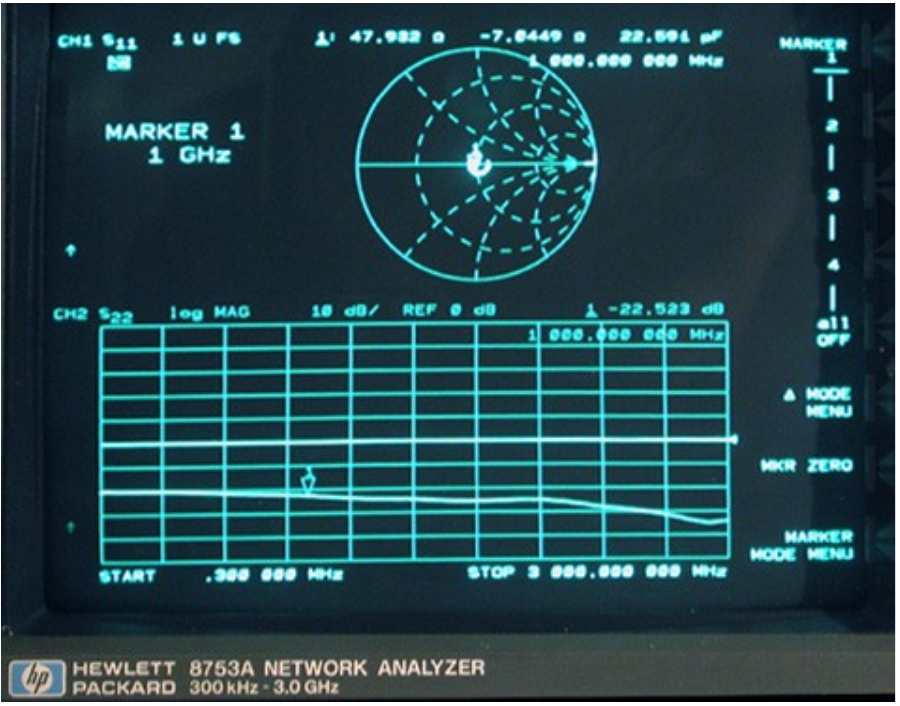
\includegraphics[width=0.6\linewidth]{images/network-analyzer-vector-graphics-display.png}
    \caption{A vector graphics display on a network analyzer\cite{assignment-text}.}
    \label{fig:vector-display-network-analyzer}
\end{figure}

\section{Vector Graphics - A Short Introduction}
Vector graphics expresses the contents of an image by using primitives, which are defined mathematically.
Primitives can be objects like lines (defined by their endpoints), squares (defined as a bounding box of two points) or curves (defined by the position of control points).
Special curves, called bézier curves, can be used to obtain complex, vectorized shapes.
The points are relative to the coordinate system of a 'scene', which is an abstract representation of an image.
Scenes are not tied to any specific physical screen resolution, but can be scaled to fit any resolution without loss of detail.

The major advantages of vector graphics are expressiveness and scalability.
Modern computing devices come in many sizes and aspect ratios.
With raster based solutions, graphics have to be regenerated for each new display size.
A vector based solution is inherently resolution independent, allowing for asset reuse across devices.

More information about vector and raster graphics is found in chapter \ref{chp:background}.

\section{Requirements}
\label{sec:requirements}
The group decided on a set of functional requirements based on initial research, listed in table \ref{tbl:func_req}.
Non-functional requirements given in the assignment text are listed in list \ref{lst:non_func_req}.

\begin{table}[h!]
\resizebox{\textwidth}{!}{
    \begin{tabular}{|l|l|}
        \hline
        \textbf{Requirement}                                                    & \textbf{Priority} \\ \hline
        The system should be able to produce and process vector primitives      & High     \\ \hline
        The system should display primitives on an vector display               & High     \\ \hline
        The system should support both straight lines and general bézier curves & High     \\ \hline
        The processor should be general                                         & High     \\ \hline
        The system should support modification of primitives                    & Medium   \\ \hline
        The system should rasterize primitives and support HDMI as an output    & Medium   \\ \hline
        A toolchain supporting the system should be available                   & Low      \\ \hline
    \end{tabular}
}
    \caption{Functional requirements.}
    \label{tbl:func_req}
\end{table}


\begin{table}[h!]
\resizebox{\textwidth}{!}{
    \begin{tabular}{|l|l|}
     	\hline															    	
        \textbf{Requirement}    												& \textbf{Priority} \\ \hline
        The processor should be implemented on a Xilinx FPGA								& High 	\\ \hline
        The unit must utilize a Silicon Labs EFM32 microcontroller to act as an				& High 	\\ 
        I/O processor 																		&   	\\ \hline
        The budget of 10 000 NOK should cover components and PCB production					& High 	\\ \hline
    
    \end{tabular}
}
    \caption{Non-functional requirements.}
    \label{tbl:non_func_req}
\end{table}


\section{A Vector Graphics Computer Architecture}

\begin{figure}[H]
    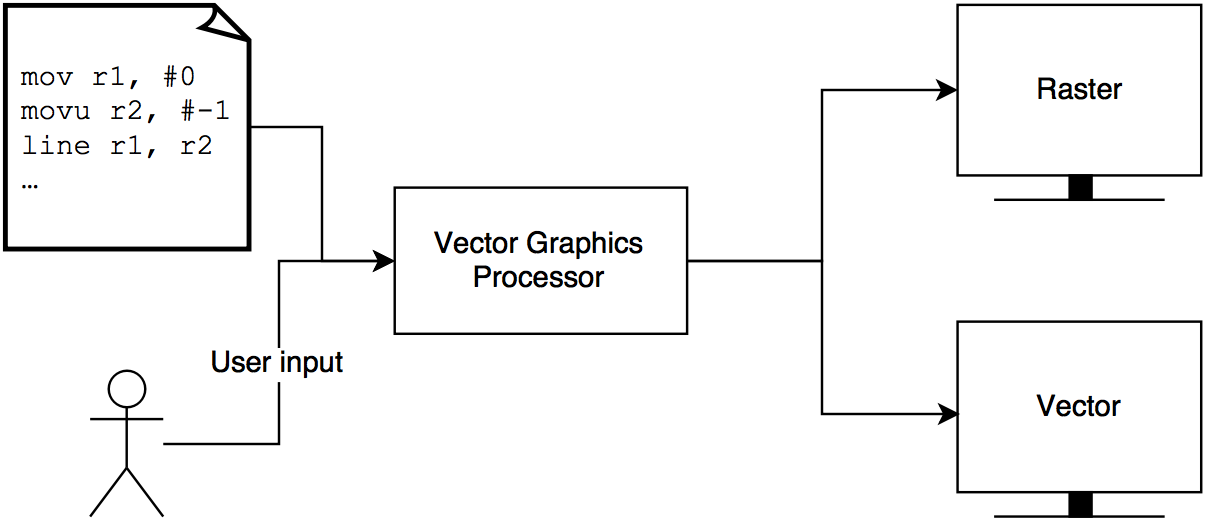
\includegraphics[width=\linewidth]{images/high_level_io.png}
    \caption{I/O overview.}
    \label{fig:io-overview}
\end{figure}

Based on the requirements, the group chose to make a general purpose computer with support for producing and processing vector graphics.
The computer would read instructions from memory, execute them on a processor core and render vector based scenes to different outputs.
To showcase the nature of vector graphics, a vector display in the form of an oscilloscope was chosen as the primary output device.
HDMI was included as secondary output to a raster display.
As a whole, the system should be assembled on a custom PCB, with the microcontroller serving as an I/O-unit while the main processor architecture and output-modules should be implemented on the \gls{fpga}.

\section{Lab Environment}
The NTNU Computer Design Lab was used frequently for this project.
The lab contains a wide variety of oscillators, signal generators and logic analyzers, which was used to test different parts of the system.
The lab also contains soldering equipment and aids - which was used extensively by the team when soldering the PCB - as well as loads of assorted electronic components.

A second lab at NTNU, ITV-458, was used by the team when programming the solution.
The lab contains computers running Ubuntu and tools for working with FPGAs.

\section{About this report}
This report is meant to give a thorough understanding of the system designed by the group.
Having introduced the assignment and described a very abstracted architecture, the next chapters introduces the system created by the group as well as give some background on computer graphics and a theoretical overview of vector graphics.

Part two presents the designed architecture in detail, outlines the programming model and elaborates on the implementation of specific subparts of the system.

Finally, part three presents performed tests, results, discussion and a conclusion.

\section{Conventions}
// TODO: Describe any conventions used in the report.
This report should be read with the following considerations in mind:

\begin{description}
    \item[group and team] 'The group' refers to everyone working on this project. The main work loads (System architecture, I/O and PCB design), were split among smaller teams. 'The team' refers to the team responsible for this functionality.
\end{description}

\chapter{Background and Theory}

Vector graphics have been popular in the computer industry for many years, seeing frequent use in analogue oscilloscopes, video arcade games \cite{astroids}, and as display devices for computers \cite{ibm2250}.

\section{Vector Graphics}

With vector graphics, mathematical expressions are used to describe an image.
The image, or the scene, is made up of primitives that describe paths and curves in order to create more complex shapes.

Vector graphics are predominantly used in 2D graphics, and is called vector graphics in order to distinguish from 2D raster graphics. In 3D graphics the internal representation of the world is usually described with vector primitives (points that form triangle surfaces for example). TODO: Some citation.

Some computer font types, like TrueType uses vector graphics and more specifically Bézier curves to represent glyphs\cite{truetype}.


TODO: Make coherent.


\section{Vector Monitor}
A vector display or monitor, is a device that draws graphics from point to point. A vector monitor utilizes CRT (Cathode Ray Tube) technology, which contain one or more electron guns and a phosphorescent screen to view images. The electron beam is deflected horizontally and vertically using electrostatic deflection. \cite{vector-monitor}

Unlike the CRT raster displays (old television sets or computer monitors), a vector monitor does not scan repeatedly in a fixed pattern. Instead it draws a point based on two voltages, one for horizontal placement and one for vertical.

One of the major advantages with vector monitors is that, since they are able to draw directly from one point to another, they do not suffer from artefacts like aliasing and pixelation. The drawback however is its inability to fill shapes in an efficient way. Therefore, vector monitors usually only draw the outline of shapes.


\section{Drawing to a oscilloscope}
As vector monitors are no longer a easily available, we need an alternative method of displaying vector graphics. It is possible to modify a CRT monitor, so that it one can manually control the deflectors, but this is quite cumbersome. The other method is using an oscilloscope, which gives an easy interface to these deflectors. This section will explain how to use the oscilloscope as a vector monitor.


To be able to draw to a oscilloscope, the oscilloscope must support at least two input channels, and the ability to draw in X-Y mode. In X-Y mode, two of the input channels (usually Ch1 and Ch2) governs the electron ray deflectors. If the channels are provided a constant voltage, a dot will be displayed on the screen, in contrast to normal mode, where  a line would be drawn.

The voltage on channel 1 will normally decide the beam's horizontal position, and channel two, its vertical position. To draw a line on the oscilloscope, one would need to repeatedly change the voltage of one or both channels back and forth.  Changing the voltage on only one channel will produce a horizontal or vertical line. 



% Part II
\part{Implementation}
\chapter{Methodology}


% Part III
\part{Results}
\chapter{Testing}
This chapter will present the testing performed on the system. It will explain the methods we used and some of the results.

\section{IO Tests}
Before our PCB board arrived we tested each subsystem separately.
During testing the group gained valuable experience about all the subcomponents and how they interacted with each others.

\subsection{DAC}

\subsubsection{Without the PCB}

The DAC was tested prior to PCB arrival, to ensure correct operation from an FPGA.
Eight wires were soldered onto the DAC, and connected to a breadboard.
The FPGA was flashed with and simple architecture, which repeatedly read the status of 14? general I/O pins, and shifted each bit out sequentially on another pin.
Both the DAC and FPGA clock input was driven by an external frequency generator, producing 3.3VPP at 10MHz.

To validate the signal output from the FPGA a logical analyser was used.

With VRef and VDD at 5.0V, the analogue DAC output was measured to 0.69V when no data signal was asserted, and 2.8V when the MSB was asserted. This small offset, is the result of some of the lower order bits being left unconnected.

\subsubsection{With the PCB}

Once the the PCB arrived we were able to test the DACs soldered onto the PCB as well as with actual data from the FPGA.

Clocking data from the FPGA to the DACs on our PCB presented some issues as we hit a limit in the Spartan 6 architecture regarding clock routing. This was resolved by using an ODDR in order to forward the clock signal to the desired output pin. //TODO: Ref for ODDR

Once we had the data input to the DACs working we could test the outputs. In does this we found some issues with out ground planes as well as the maximum output voltages from the DACs. The maximum voltage we were able to get was 1.6V, a little under half of our reference voltage of 3.3V. //TODO: Update this when the problem is fixed.


\subsection{Oscilloscope}
As a proof of concept to draw on an oscilloscope, we created a 4-bit resistor ladder DAC. The schematic of the DAC is displayed in Figure \ref{fig:r2r-ladder}.
An Arduino was used to control the DAC.

To test drawing on both x-axis and y-axis, the circuit consisted of 2 4-bit DACs.
With a small Arduino program we were able to draw a square, depicted in Figure \ref{fig:osc_poc}.
When the Arduino changed the voltage on its GPIO pins, there was a voltage drop across all pins.
The consequence of the voltage drop is clearly visible (see Figure \ref{fig:osc_poc}).


\begin{figure}[h]
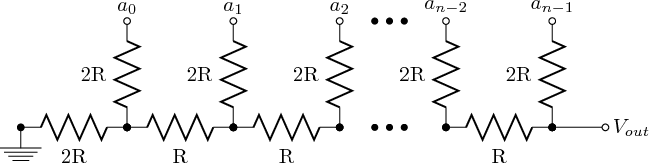
\includegraphics[width=\columnwidth]{images/r2r-ladder}
\centering
\caption{Schematics of the resistor-ladder\cite{r2r-ladder-schematics}.}
\label{fig:r2r-ladder}
\end{figure}

\begin{figure}[h]
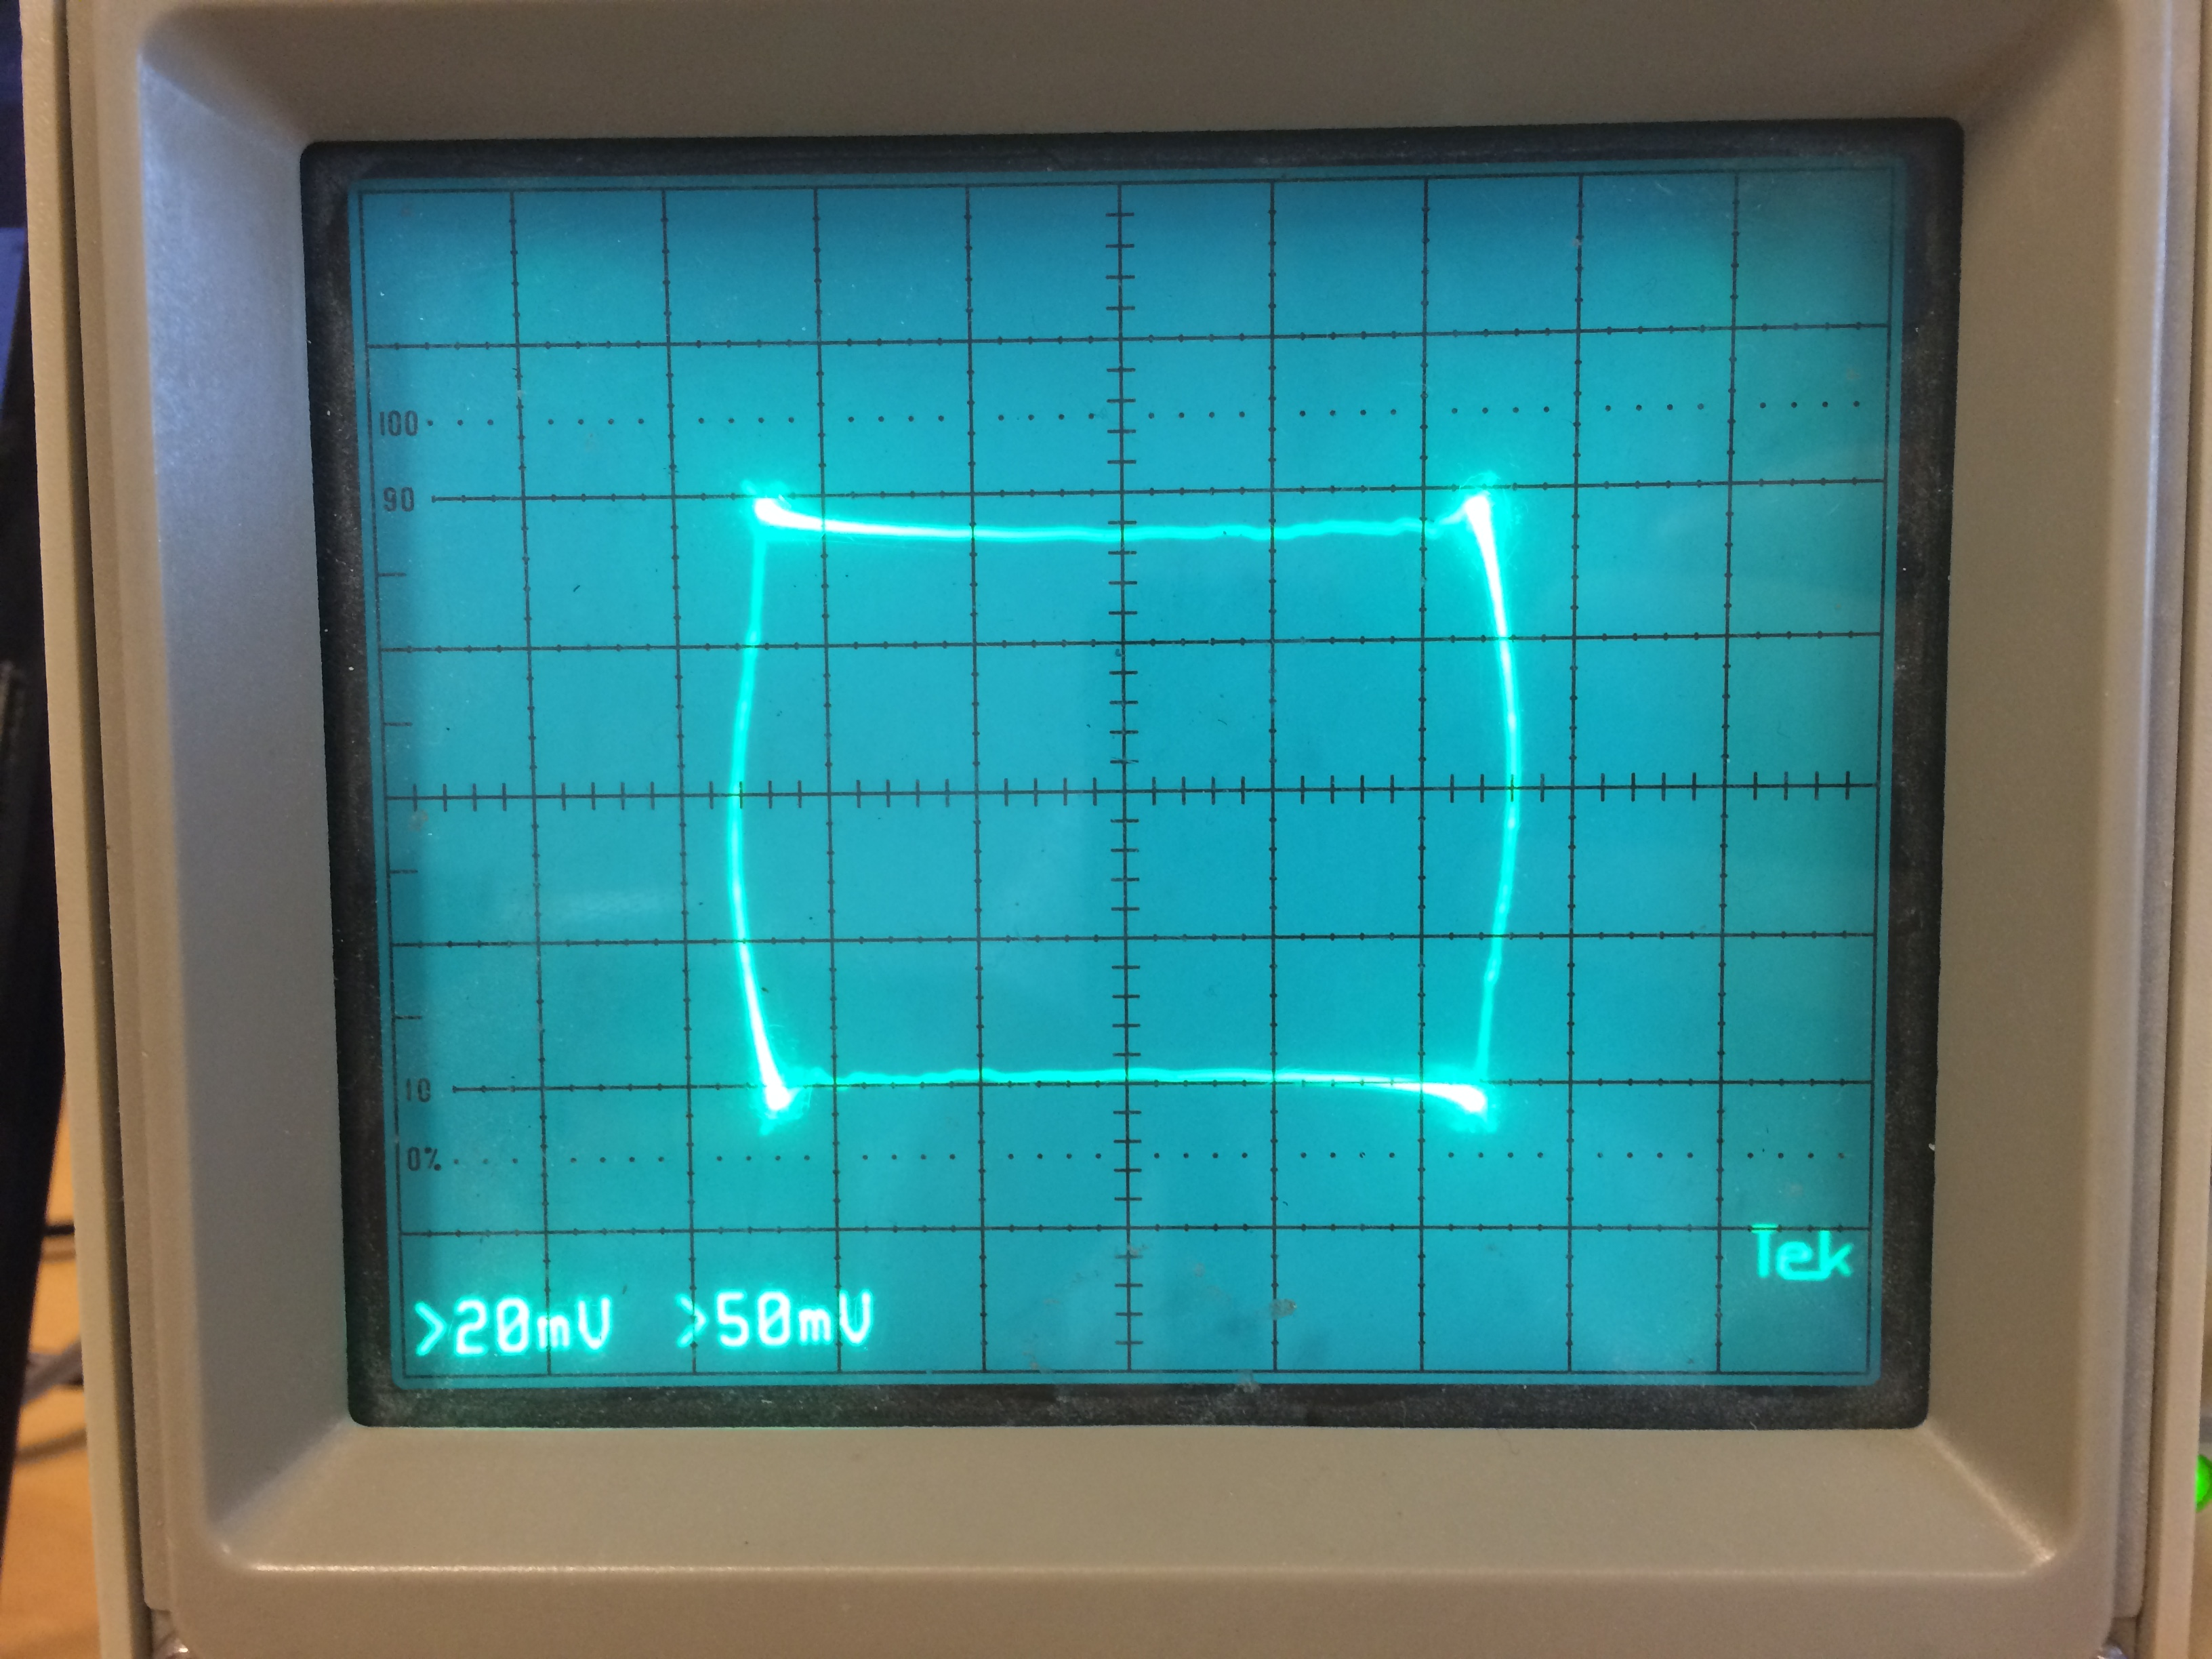
\includegraphics[width=\columnwidth]{images/osc_square_close}
\centering
\caption{A "square" drawn on the oscilloscope using an Arduino and two resistor-ladder DACs}
\label{fig:osc_poc}
\end{figure}

\section{Physical PCB and Components testing}

// TODO: Restructure this, some of it belongs in results, some in discussion.

When we had received the PCB and the components, we had to make sure that every component worked properly independent of the PCB, then testing if they worked on the PCB. Many major components were impossible to test without soldering on the PCB though. Examples were the FPGA and MCU, because of their tiny ball grid pins.

\subsection{Soldering}
There were different ways of soldering components on the PCB. It depended on components being through hole, surface mounted, pin size, etc.
\subsubsection{Ball Grid Arrays (BGA)}
Both the FPGA and MCU were ball grid arrays.
Therefore, they were soldered on the PCB,//TODO: No paste were smeard by smearing paste over the corresponding area, putting them carefully on, and putting the PCB in a heater. The heater made the components stick properly to the paste. This was the only way, since soldering pins directly under the component by hand, isn't practically possible.

\subsubsection{Surface Mounted Components}
Most surface mounted components where the pins weren't too small and crowded, were soldered by hand. Paste were used before hand, just like with BGAs, but after that the pins could be soldered by hand, since the pins were within physical reach. 
\newline
If pins were too small and tight, the same technique was used as for the BGAs.

\subsubsection{Through Hole Components}
Through Hole components were the easiest to solder, since the pin size and the space between them was relatively large. Additionally they were on the bottom side of the board. No paste was needed, each individual pin could be soldered with tin wires.

\subsection{Testing}
We had to find and fix all errors and faults with our PCB design and components, that were a hazard to our desired resulting system.  
We ran tests during our soldering process to make sure the system so far worked desirably. Running tests during the process, lowered the amount of potential sources of errors, which made it easier to discover errors.

\subsubsection{Power Planes}
It was very important to verify that the power planes worked as we intended. Obviously, nothing would work without power. Hence, this was the very first test we performed.
\newline
Everything necessary for power to be present, was soldered on. This included power headers, and the 3.3 voltage regulator. External power was inserted through power headers. By measuring different places with a voltmeter, we already discovered anomalies. The voltmeter showed only 2.3V instead of 3.3V. Further testing revealed that one of the voltage regulator pins hadn't been soldered properly, resulting in a loss of 1V. After fixing this, the digital VCC plane contained the correct 3.3V.


\section{PCB Design Flaws}
No project would be complete without something going wrong. Our project is no exception. After receiving our manufactured PCB, we started to discover various complications. This section discusses the more serious ones in detail, and what we did to solve the problem.

\subsection{Incorrect Wiring}
We discovered that our buttons was wired wrong, since they caused short-circuits. The reason was sloppy study of the datasheet, as shown in figure \ref{fig:Button Issue}. Luckily, this could be remedied by rotating the button 90 degrees, if we adjusted the physical connectors to fit the footprint.

\begin{figure}[h!]
\centering
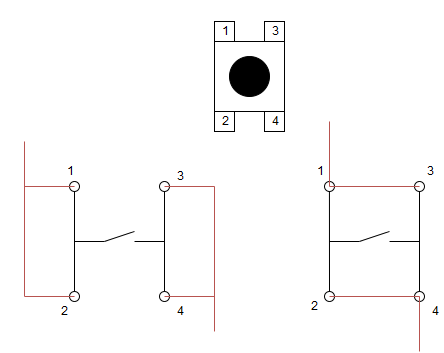
\includegraphics[scale=0.5]{images/Button_Issue.png}
\caption{Top figure shows the button as it looks like on the PCB. On the left: Correct wiring according to datasheet. On the right: Incorrect wiring leading to short-circuit}
\label{fig:Button Issue}
\end{figure}

When testing the oscillators, they did not seem to work. The datasheet for these components clearly stated that connecting the E/D pin to either 'No Connect' or '1' equaled active, so we did not connect it. We tried to remedy by connecting E/D to Vcc, and the problem was solved.
\newline
\newline
The Vref chip was supplied with 3.3V, but should have been supplied with analogue 5V instead. This could be remedied by cutting on the 3.3V power trace, since the trace is located on the top layer and no other traces are beneath it. Then we could connect analogue 5V via header from the voltage regulator to the input pin on the Vref chip.
\newline
The DACs were supplied with analogue 5V, but should have been supplied with 3.3V. The analogue 5V should go to the Vref chip instead. Solved by switching the two connections.

\subsection{PCB Placement and Footprints}
The BNC connector's footprint was wrongly routed - ground and Vcc was switched on the PCB. We discussed inverting the signal, but found that switching the pins on the component was the easiest thing to do.
\newline
\newline
It would have been beneficial if we had placed the 3.3V voltage regulator closer to the JTAG debugging port, since the Xilinx JTAG platform cable required a 3.3V power supply.
\newline
\newline
The micro USB footprint originally contained mounting holes, but were wrongly removed before manufacturing. Luckily, these did not act as connectors, and we could therefore solder the USB receptacle onto the PCB like a surface mount component.

\subsection{Component Order Issues}
The initial LEDs we ordered were reverse mounted, meaning that they required a hole in the board and had to be soldered on to the bottom layer. Because of this, we had to buy some new ones.
\newline
\newline

\subsection{Component sizes}
In hindsight, it would have been better to order bigger components. Since this is a prototype board where we mostly solder by hand, an increase in size would only be beneficial for us. If the project should go into large scale production, we could have tried to shrink the size.





% Part IV
\part{Appendices}

% Bibliography - edit references.bib and use the \cite command in text
\bibliographystyle{plain}
\bibliography{references}
\end{document}
